\documentclass[10pt,a4paper]{article}
\usepackage[utf8]{inputenc}
\usepackage[spanish]{babel}
\usepackage{amsmath}
\usepackage{amsfonts}
\usepackage{amssymb}
\usepackage{graphicx}
\author{Markus Fischer • Guzmán López • David Pérez • Ander Raso}
\title{Proyecto de Minería de Datos: \linebreak Borrador de memoria completa}
\date{}

%Borrador de la memoria completa: estructura con todas las secciones y en cada sección esquema del contenido
%
%    1. Introducción completa
%        1.1 En qué consiste la tarea
%        1.2 Qué retos presenta
%        1.3 Propuesta para abordarlos
%    2. Descripción y análisis de datos completo
%    3. Pre-proceso: describir en qué consiste, fase de limpieza de datos, qué rutinas se han aplicado para cambiar el formato de datos de texto a un vector numérico
%    4. Clustering: Algoritmo de clustering en pseudo-código.
%    5. Evaluación: ¿Qué técnicas de evaluación se emplearán? Detallar formalismo teórico
%    6. Detalle de los experimentos que se van a realizar y el objetivo de cada experimento
%    7. Conclusiones y trabajo futuro: vacío hasta completar trabajo
%    8. Bibliografía

\begin{document}
\maketitle
\newpage

\tableofcontents
\newpage

\section{Introducción}
	\subsection{Objetivo de la tarea}
	En este proyecto se nos encarga la tarea de trabajar en el campo del \textit{Text Mining} y del clustering de documentos. Nuestro objetivo es, a partir de una gran colección de textos, buscar formas de agruparlos y tratar de extraer conclusiones de los resultados que obtengamos.
	\subsection{Propuesta de trabajo del grupo}
	Como grupo, hemos decidido realizar la tarea sobre la colección de autopsias verbales que se propuso como opción. Esto se debe a que, ademas de considerar el tema muy interesante, creemos que es una propuesta que se encuentra muy próxima al uso que se da al \textit{Text Mining} en el ámbito científico.\\
	
    Sin embargo, de esta decisión también surgen ciertos retos a los que debemos poner solución:
	\begin{itemize}
	\item Muchos de los reportes de autopsia están en un lenguaje poco preciso y muchas veces ininteligible, probablemente causado tanto por el desconocimiento de los que dieron el reporte, como por las traducciones que se han hecho a estos.
	\item En muchas ocasiones no hay reporte verbal o este es irrelevante, por lo que la única información útil de que se dispone es de los datos del difunto, tales como país, edad, sexo, etc.
	%TODO: Añadir alguna más para que no quede vacío.
	\end{itemize}

\section{Descripción y análisis de datos}
En este proyecto vamos a trabajar con autopsias verbales. Éstas son reportes que dan familiares o personas cercanas a un fallecido en lugares donde por norma general no se realiza una autopsia post-mortem a menos que sea estrictamente necesario. Estas autopsias se componen de información básica del paciente (edad, sexo, etc) así como del reporte oral que ha dado el relativo al que se ha entrevistado.\\

La base de datos de las autopsias verbales se compone de casi 12000 instancias. En cada instancia disponemos de una serie de atributos:

\begin{itemize}
\item \textbf{newid:} Identificador númerico de la instancia.
\item \textbf{module:} Grupo de edad del fallecido. Los valores posibles son ``neonate'', ``child'' y ``adult'' (Fig: \ref{fig:age_graph}). 

\item \textbf{site:} Lugar del que proviene la autopsia: los valores posibles para este campo son (Fig: \ref{fig:loc_graph}): 
    \begin{itemize}
    \item AP=Andhra Pradesh, India
    \item Dar=Dar es Salaam, Tanzania
    \item UP=Uttar Pradesh, India
    \item Pemba=Pemba, Tanzania
    \item Bohol=Bohol, Philippines
    \item Mexico=Distrito Federal, Mexico
    \end{itemize}


\begin{figure}
  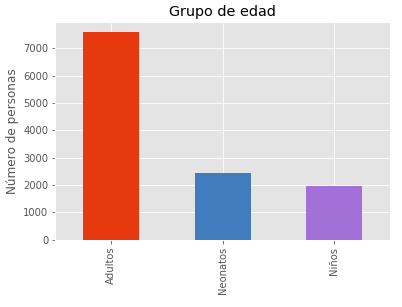
\includegraphics[width=\linewidth]{figures/plot_grupo_edad.png}
  \caption{Número de instancias según la edad del fallecido}
  \label{fig:age_graph}
\end{figure}

\begin{figure}
  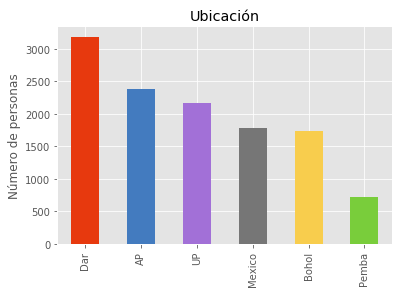
\includegraphics[width=\linewidth]{figures/plot_ubicacion.png}
  \caption{Número de instancias según la ubicación del fallecido}
  \label{fig:loc_graph}
\end{figure}  

\begin{figure}
  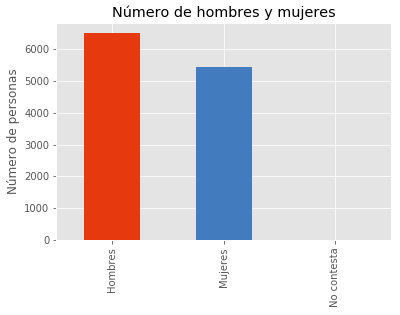
\includegraphics[width=\linewidth]{figures/plot_sexo.png}
  \caption{Número de instancias según el sexo del fallecido}
  \label{fig:sex_graph}
\end{figure}  
    
\item \textbf{gs\_text34:} Causa de la muerte del paciente.
\item \textbf{sex:} Sexo del difunto. Los valores posibles son 1, 2, 3 y 4. Cada uno de estos valores hace referencia a ``hombre'', ``mujer'', ``se niega a responder'' y ``desconocido'' respectivamente (Fig: \ref{fig:sex_graph}).
\item \textbf{age\_years:} Edad del fallecido en años. En caso de ser igual a 999 significa que es desconocida.
\item \textbf{age\_months:} Edad del fallecido en meses. En caso de ser igual a 99 significa que es desconocida.
\item \textbf{age\_days:} Edad del fallecido en días. En caso de ser igual a 99 significa que es desconocida.
\item \textbf{open\_response:} Declaración de la persona cercana al difunto en caso de que hubiese una. En este texto se han eliminado todas las referencias que se diesen en la declaración que pudiesen relacionarse con el difunto para asegurar su privacidad, tales como menciones a los lugares y hospitales en los que se ha encontrado, el nombre de personas o fechas concretas en relación al fallecido, etc. En su lugar se han sustituído por palabras neutrales entre corchetes, tales como ``[PERSON]'' o ``[HOSPITAL]''.
\end{itemize}

\section{Preproceso de datos}
El formato original del archivo de autopsias es un xlsx, es decir, una hoja de cálculo de Microsoft Office. Esto nos facilita mucho la tarea de procesar los textos, ya que es muy fácil convertir de xlsx a formatos de texto plano. En nuestro caso elegimos csv, ya que es un formato muy limpio y que más adelante nos será útil para transformarlo al formato arff, el cual es compatible con Weka y gran parte de las librerias de Data Mining que hemos utilizado.\\

\subsection{Limpeza de textos}
Una vez tenemos nuestro documento como csv, procedemos a preprocesarlo. Ya que los valores identificador, grupo de edad, lugar, diagnóstico, sexo y edad están codificados segun unos criterios que se mantienen a lo largo de todas las instancias, sabemos que no debemos preprocesarlos. Sin embargo, es en el campo de la respuesta verbal en el que tenemos que solucionar algunas anomalías:
\begin{itemize}
\item \textbf{Mayúsculas y minúsculas:} Para evitar diferencias entre palabras escritas completamente en mínuscula, completamente en mayúscula o con la primera letra mayúscula, debemos transformar todas ellas a un mismo formato. En nuestro caso el formato escogido son las minúsculas.
\item \textbf{Saltos de línea:} En algunos casos nos encontramos con saltos de línea internos en el texto. Ya que csv separa sus diferentes atributos por comas y las instancias por líneas, los saltos de línea internos en el texto crean inconsistencias y errores al procesar el csv. El método más fácil para deshacerse de ellos pero mantener el texto en el mismo formato es sustituírlos por espacios.
\item \textbf{Números:} Los números, pese a ser uno de los elementos más comunes en los textos, han sido uno de los más díficiles de preprocesar, no por su dificultad en cuanto a programar, sino a la decisión que tomar en cuanto a ellos. Esto se debe a que se toman como una palabra por si mismos y pese a tener un peso informativo alto, sólo es así cuando va acompañado de otra palabra a la que calificar. Ya que los programas de text mining los van a considerar independientes del resto de palabras, hemos considerado que la información que van a aportar es suficientemente baja como para simplemente eliminarlos del texto.
\item \textbf{Tokens:} Se consideran tokens a todas las palabras recurrentes que no tienen ni significado ni peso informativo, como por ejemplo ``the'' o ``a''. Mediante un diccionario de tokens en la lengua inglesa hemos podido detectar todos ellos y eliminarlos del texto.
\item \textbf{Símbolos:} Aquí tenemos varios problemas que debemos arreglar de diferentes formas.
\begin{itemize} 
\item \textbf{Barras ``/'':} En ocasiones nos encontramos con dos palabras escritas de modo "palabra1/palabra2". Para evitar que se procesen ambas como una misma palabra, realizamos el mismo procedimiento que utilizamos con los saltos de línea: cambiamos las barras por espacios.
\item \textbf{Corchetes ``[ ]'':} En gran parte de las instancias que disponen de autopsia verbal nos encontramos con referencias a nombres de personas, hospitales, años concretos, etc. Para preservar la privacidad de los fallecidos y sus relativos estos han sido sustituídos por sus correspondientes palabras clave entre corchetes, como por ejemplo ``[PATIENT]'' o ``[HOSPITAL]''. Ya que estos datos son en la inmensa mayoría de casos de poca utilidad, hemos decidido que estás palabras serán completamente eliminadas de los textos.
\end{itemize}
\end{itemize}

\subsection{\textit{Word vector}}
Después de limpiar los textos de las instancias necesitamos convertir ese texto a un formato que podamos utilizar. El formato escogido es el TF-IDF, el cual consiste en una representación vectorial del conjunto de palabras presentes en todos los documentos (instancias). Cada una de las palabras se evalúa individualmente y se le asigna un valor numérico en función al número de apariciones que tiene en cada documento, pero teniendo en cuenta también en cuántos de los documentos aparece para evitar darle excesiva importancia a palabras que simplemente se repiten por ser comunes.\\

Escogimos la representación TF-IDF en favor de \textit{Bag of Words} por el hecho de que aporta más información. \textit{Bag of Words} se limita a inicar la presencia o ausencia de palabras en los documentos mientras que TF-IDF le asigna un valor en función de su aparente importancia teniendo en cuenta todos los documentos.

\section{Clustering}
Para el clustering hemos decidido utilizar el algoritmo K-Means, el cual implementaremos en Java. Opciones para el algoritmo a tener en cuenta y que faltan por implementar son:

\begin{itemize}
\item \textbf{inicialización de los centroides:} hay varias formas de elegir los valores iniciales de los centroides, su inicialización puede tener un gran efecto en los resultados.
    \begin{itemize}
    \item inicialización a instancias aleatorias.
    \item inicialización variaciones aleatorias de la media del conjunto de instancias.
    \item inicialización a partir de un clustering previo.
    \end{itemize}
\item \textbf{obtención de las distancias:} la fórmula para calcular la distancia será la distancia Minkowski, con \(m \in \Re\). \(m=1\) es la distancia Manhattan y \(m=2\) es la distancia Euclidea.
\item \textbf{definición de distancia \textit{inter-cluster}:} también hay varias formas para buscar la distancia entre dos clusters distintos. En este caso, vamos atrabajar con dos:
    \begin{itemize}
    \item \textit{complete-link}. La distancia entre dos clusters es igual a la distancia entre las dos instancias, una de cada cluster, más lejanas entre sí.
    \textit{single-link}. La distancia entre dos clusters es igual a la distancia entre las dos instancias, una de cada cluster, más cercanas entre sí.
    \end{itemize}

\end{itemize}

\subsection{Representación gráfica}
Una vez que tenemos las instancias separadas en clusters, sería interesante representarlas gráficamente para poder ver como se relacionan los clusters, calculados a partir del texto describiendo la enfermedad, con la causa de la muerte anotada en las autopsias. Para ello, tenemos que reducir el enorme espacio de atributos de las instancias a algo que podamos representar en un espacio de no más de tres dimensiones. Para ello pensamos en utilizar el método PCA (\textit{Principal Components}) que hace precisamente eso: reduce un gran número de variables a una serie de valores representativos, ortogonales entre sí para representarlos en espacios de pocas dimensiones.\\

Sin embargo nos encontramos con un problema: el PCA es un método costoso, tanto en tiempo como en uso de memoria. Al tratar de aplicar el PCA a nunestro conjunto de casi 12000 instancias, y teniendo alrededor de 8000 atributos en cada una de ellas (a causa del formato TF-IDF) el programa no fue capaz de terminar el proceso, siempre resultando en una falta de memoria, sin importar le permitiesemos utilizar.\\

Pensamos en llevar a cabo el PCA individualmente en cada clusters, dividiendo la carga en distintos intentos, pero como el PCA utiliza todo el conjunto para determinar los componentes principales, creemos que realizar el proceso en cada cluster de forma separada en lugar de sobre todo el conjunto podría causa inconsistencias a la hora de reducir los vectores.

\section{Evaluación}

% TODO: está poniendo estas imágenes como le da la gana. - Ander

\begin{figure}[h] % sin esta "h" la figura se va a la seccion anterior ¿?
  \centerline{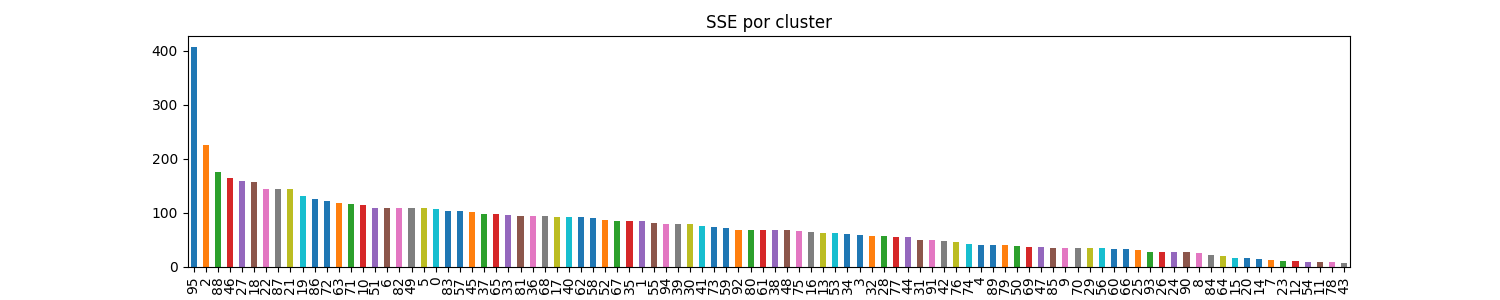
\includegraphics[scale=.6]{figures/sse_plot.png}}
  \caption{SSE por cluster}
  \label{fig:sse_graph}
\end{figure} 

\begin{figure}[h]
  \centerline{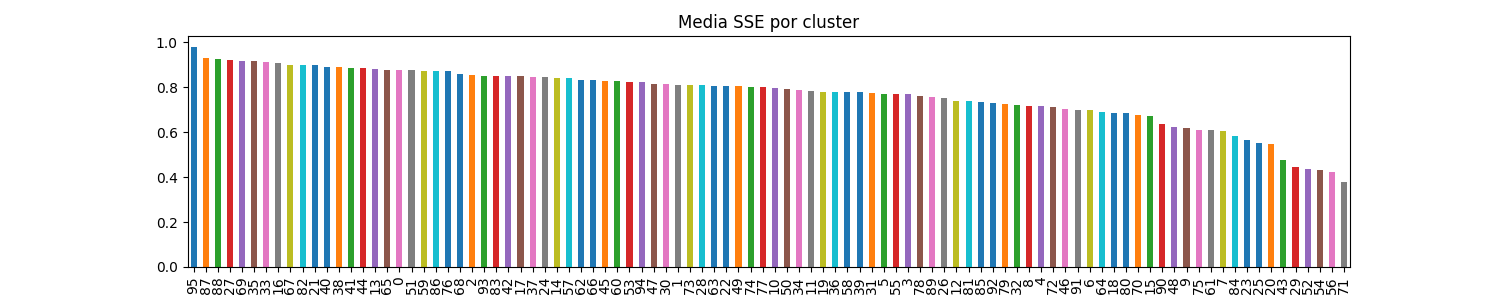
\includegraphics[scale=.6]{figures/sse_avg_plot.png}}
  \caption{Media del SSE por cluster}
  \label{fig:sse_avg_graph}
\end{figure} 

\begin{figure}[h]
  \leftskip-3.5cm
  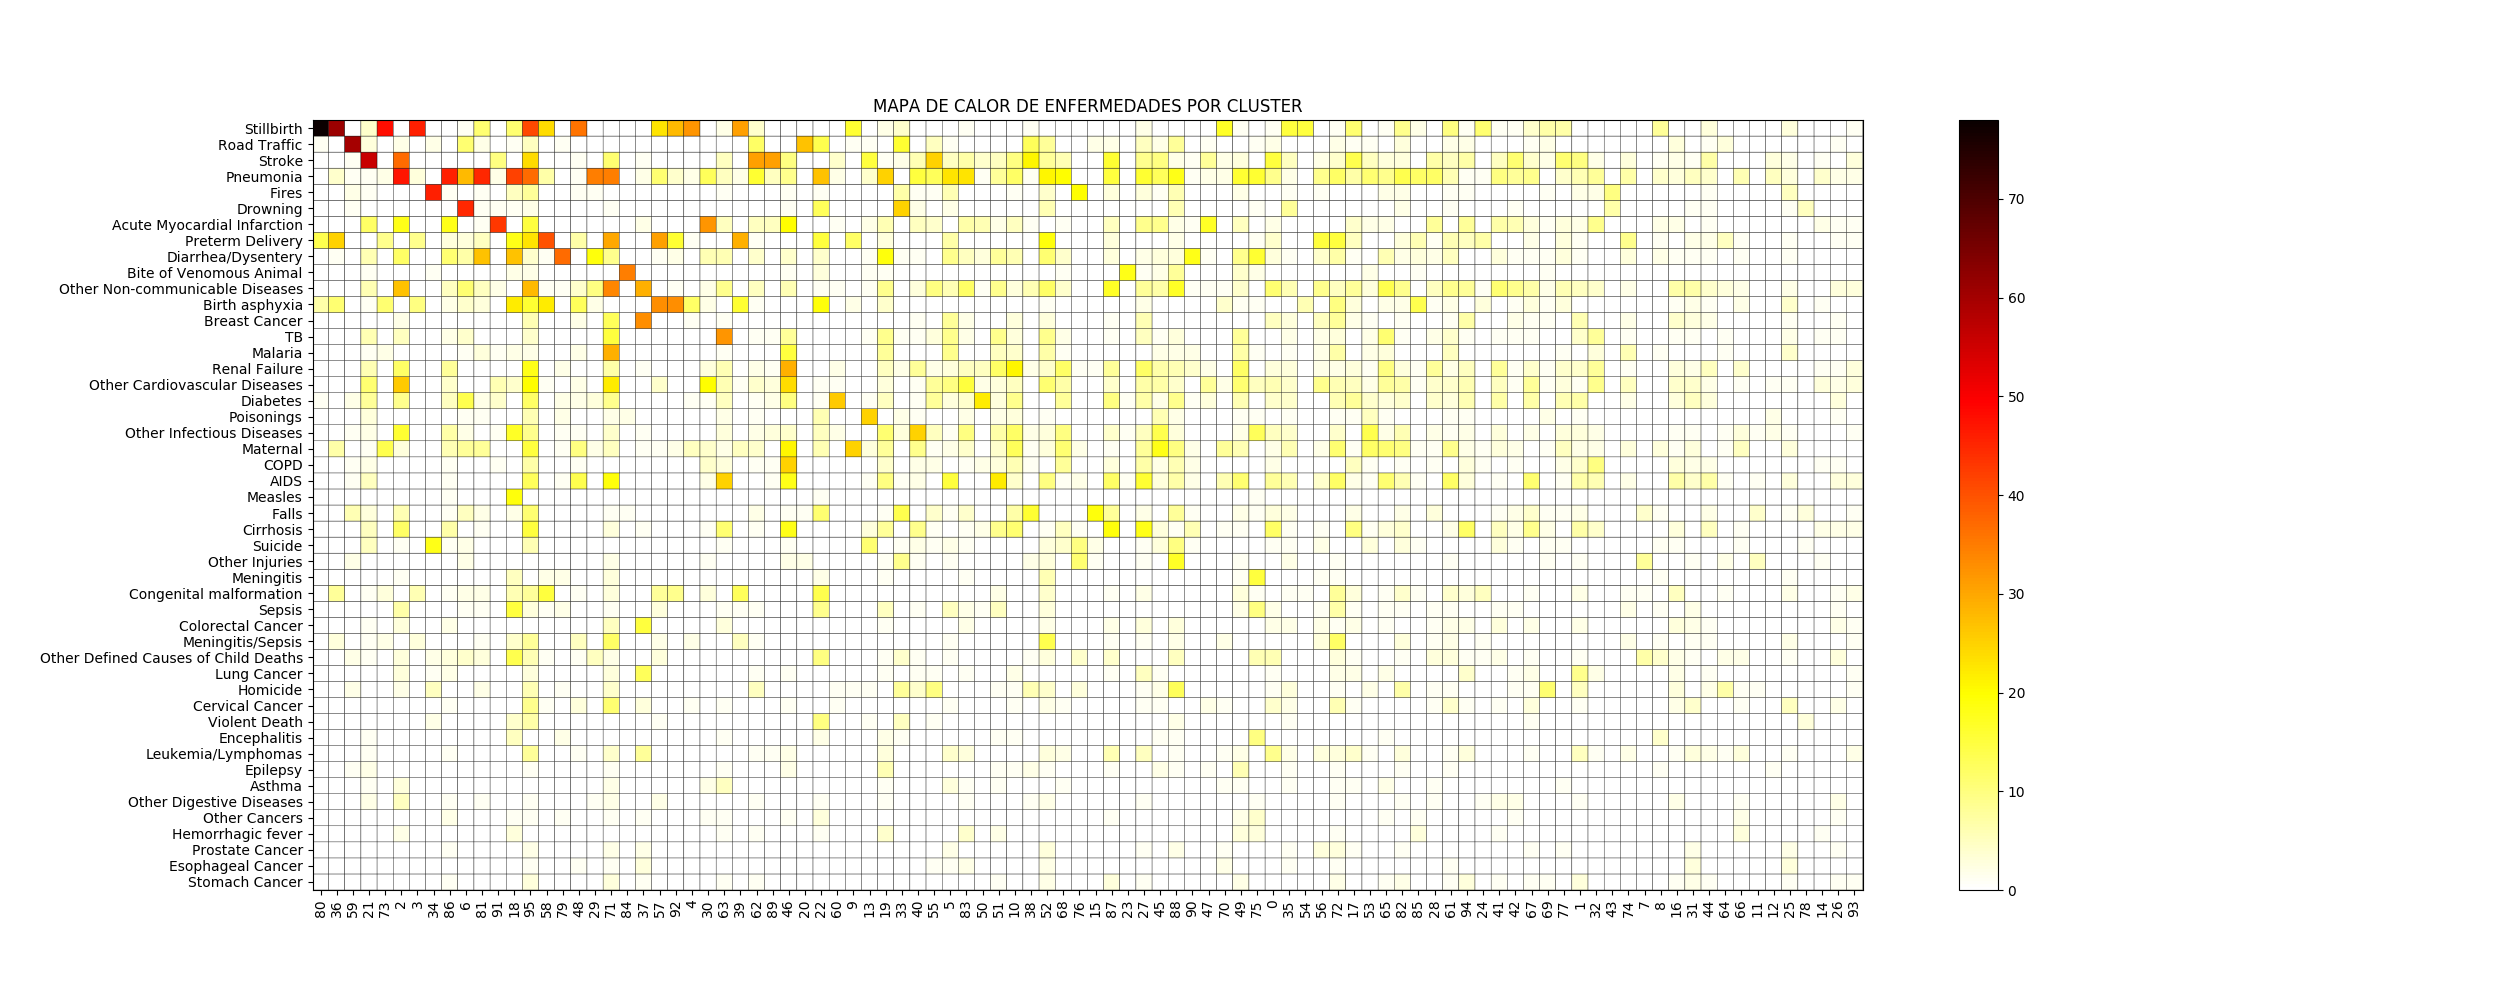
\includegraphics[scale=0.37]{figures/heatmap.png}
  \caption{Mapa de calor de las enfermedades por cluster}
  \label{fig:heatmap_graph}
\end{figure}

Como se puede observar en la figura \ref{fig:heatmap_graph}, hemos realizado un mapa de calor para poder ver de una forma más clara las enfermedades que han sido agrupadas en cada cluster. Considerando las casillas que contienen un mayor valor hemos ordenado las columnas de izquierda a derecha y las filas de arriba a abajo. De esta manera tenemos organizados en la diagonal los clusters más específicos. Si examinamos el resultado final son interesantes los siguientes clusters:

\begin{itemize}
\item \textbf{Cluster 80:} este cluster ha agrupado mayormente \textit{stillbirt} y en mucha menor medida \textit{preterm delivery} y \textit{birh asphyxia} que también están relacionadas con el embarazo
\item \textbf{Cluster 36:} es muy parecido al cluster 80 pero este tiene menos \textit{stillbirt} aunque muchos más \textit{preterm delivery} y \textit{birth asphyxia}. Además, también se encuentran \textit{maternal} y \textit{congenital marformation} lo que en definitiva lo hace un cluster muy interesante para agrupar causas de muerte relacionadas con el embarazo.
\item \textbf{Cluster 59:} se encuentran sobre todo \textit{road traffic} y en menor cantidad \textit{falls}. Este cluster ha sido capaz de agrupar causas de muerte relacionadas con accidentes.
\item \textbf{Cluster 21:} las causas de muerte con mayor número de casos de este cluster han sido \textit{stroke}, \textit{acute myocardial infarction} y \textit{other cardiovascular diseases}. Todas ellas relacionadas con enfermedades cardiovasculares pero también se encuentran en menor medida \textit{diabetes}, \textit{renal failure} y \textit{AIDS} entre otras.
\item \textbf{Cluster 34:} este es muy específico para \textit{fires}, \textit{suicide} y contiene unos pocos de \textit{homicide}.
\item \textbf{Cluster 91:} es similar al cluster 21 pero se han agrupado aquí más \textit{acute myocardial infarction} que \textit{stroke}.
\item \textbf{Cluster 79:} sobre todo encontramos \textit{diarrhea/disentery}. Ha sido muy específico.
\item \textbf{Cluster 84:} principalmente se haya \textit{bite of venomous animal}.
\item \textbf{Cluster 57 y 92:} han agrupado casos que tienen que ver con el embarazo como lo ha hecho el cluster 36, pero estos lo han hecho de forma más general.

Si nos seguimos moviendo por las columnas de la derecha vemos clusters en los que no predomina una causa de muerte y empiezan a agrupar cada vez más causas diferentes que no parecen estar relacionadas.

\end{itemize}




%\section{Experimentos}
%\section{Conclusiones}

%\section{Bibliografía}

\end{document}
